
\documentclass{beamer}
\mode<presentation>
\usepackage{amsmath}
\usepackage{amssymb}
%\usepackage{advdate}
\usepackage{graphicx}
\graphicspath{{../figs/}}
\usepackage{adjustbox}
\usepackage{subcaption}
\usepackage{enumitem}
\usepackage{multicol}
\usepackage{mathtools}
\usepackage{listings}
\usepackage{url}
\def\UrlBreaks{\do\/\do-}
\usetheme{Boadilla}
\usecolortheme{lily}
\setbeamertemplate{footline}
{
  \leavevmode%
  \hbox{%
  \begin{beamercolorbox}[wd=\paperwidth,ht=2.25ex,dp=1ex,right]{author in head/foot}%
    \insertframenumber{} / \inserttotalframenumber\hspace*{2ex} 
  \end{beamercolorbox}}%
  \vskip0pt%
}
\setbeamertemplate{navigation symbols}{}
\let\solution\relax
\usepackage{gvv}
\lstset{
%language=C,
frame=single, 
breaklines=true,
columns=fullflexible
}

\numberwithin{equation}{section}
\title{6.4.1}
\author{AI25BTECH11001 - ABHISEK MOHAPATRA}
% \maketitle
% \newpage
% \bigskip
\begin{document}
{\let\newpage\relax\maketitle}
\renewcommand{\thefigure}{\theenumi}
\renewcommand{\thetable}{\theenumi}





	 	\textbf{Question}:
		Fit a straight line trend by the method of least squares and find the trend value for
the year 2008 using the data from the given table


TABLE : Show yearly trend of production of goods in lakh tonnes
\begin{table}[H]
\centering
	\begin{tabular}{|c|c|}
\hline
\text{Year} & \text{Production (in lakh tonnes)} \\ 
\hline
2001 & 30 \\
\hline
2002 & 35 \\
\hline
2003 & 36 \\
\hline
2004 & 32 \\
\hline
2005 & 37 \\
\hline
2006 & 40 \\
\hline
\end{tabular}


	\caption*{}
	\label{data}
\end{table}

%TODO Table

		\textbf{Solution:}
		Equation of a straight line be:
		\begin{align}
				y =  mx + c
		\end{align}
		\begin{align}
				y = \myvec{c&m}\myvec{1\\x}
		\end{align}
		Let this equation be 
		\begin{align}
				y = \vec{N}^\top\vec{X}
		\end{align}

		Let the given value of the years be a column vector $\vec{X_0}$ and the corresponding values of production be $\vec{D}$.


		let $\vec{X} = \myvec{\brak{1}_{n\times 1}&\vec{X_0}}$. 

		
		let $\vec{X} = \myvec{\vec{x_1}&\vec{x_2}&...&\vec{x_n}}^\top$
		and $\vec{D} = \myvec{y_1&y_2&...&y_n}^\top$
		
		so sum of the square of error = e =
		\begin{align}
				\Sigma|y_i - \vec{N}^\top\vec{x_i}|^2
		\end{align}
		\begin{align}
		=		\Sigma\brak{y_i - \vec{N}^\top\vec{x_i}}\brak{y_i - \vec{N}^\top\vec{x_i}}
		\end{align}
		\begin{align}
				=		\Sigma\brak{\brak{y_i}^2 - 2y_i^\top\vec{N}^\top\vec{x_i} + \brak{\vec{N}^\top\vec{x_i}}^2}
		\end{align}
		for this to be minimum , $\nabla_\vec{N}$ e = 0
		\begin{align}
		\nabla_{\vec{N}} e=\Sigma\brak{- 2y_i\vec{x_i} + 2\brak{\vec{N}^\top\vec{x_i}}\vec{x_i}}=0
		\end{align}
		\begin{align}
		\nabla_{\vec{N}} e=\Sigma\brak{- 2y_i\vec{x_i} + 2\brak{\vec{x_i}\vec{x_i}^\top}\vec{N}}=0
		\end{align}
		so,
		\begin{align}
				\brak{\Sigma\vec{x_i}\vec{x_i}^\top}\vec{N} = \Sigma y_i\vec{x_i}
		\end{align}Or,
		\begin{align}
				\vec{N} = \brak{\Sigma\vec{x_i}\vec{x_i}^\top}^{-1}\brak{\Sigma y_i\vec{x_i}}
		\end{align}Or,
		\begin{align}
				\vec{N} = \brak{\vec{X}^\top\vec{X}}^{-1}\brak{\vec{X}^\top\vec{D}}
		\end{align}
		Given,\begin{align}
		\vec{X} = \myvec{1&1&1&1&1&1\\2001&2002&2003&2004&2005&2006}^\top
		\end{align}
		And,\begin{align}
		\vec{D} = \myvec{30&35&36&32&37&40}^\top
		\end{align}
		\begin{align}
				\vec{X}^\top\vec{D} = \myvec{30+35+36+32+37+40 \\ 2001\times30 + ... + 2006\times40} = \myvec{210 \\ 420761}
		\end{align}
		\begin{align}
				\brak{\vec{X}^\top\vec{X}} = \myvec{6.0 & 12021.0 \\
12021.0 & 24084091.0}
		\end{align}
		\begin{align}
				\brak{\vec{X}^\top\vec{X}}^{-1} = \myvec{229372.295 & -114.485714 \\
-114.485714 & 0.0571429}
		\end{align}
		Putting the matrices,\begin{align}
				\vec{N}	= \myvec{229372.295 & -114.485714 \\
-114.485714 & 0.0571429}\myvec{210 \\ 420761} = \myvec{-2941.628571 \\
1.485714}
		\end{align}
		So,
		\begin{align}
				y = \vec{N}^\top\myvec{1\\2008} = 41.685714
		\end{align}
		Therefore, expected value is 41.685714.
	

	Graph:
\begin{figure}[h!]
	\centering
	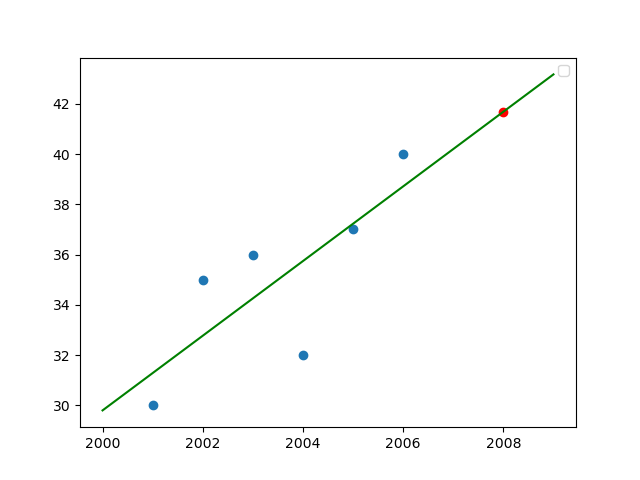
\includegraphics[width=0.7\linewidth]{img.png}
\end{figure}
\end{document}




